\section{线性叠加与相干条件}
在线性介质中，各列波可以独立传播，总位移是同一位置、同一时刻各位移的代数和。应先统一振动方向及符号，再相加函数；两列波振幅不能在任意相位下直接相加，能量也不能先按强度作简单相加。

两列同方向振动的合成，既要确定幅度，也要确定相位。稳定干涉要求频率相同、相位差在观察期间稳定；等频而相位差无规则变化时，不能形成稳定强弱分布。下面先把相位沿传播路径写清，再用正交分量求合振动。所谓相消还要求到达振幅相等，不仅是相位相反。

从两点源传播到$P$时，若源初相为$\varphi_1,\varphi_2$，则
\[
\Delta\varphi=\varphi_2-\varphi_1-k(r_2-r_1).
\]
同相源才可以直接用整波长程差判增强、半奇数波长程差判减弱。反相源的结论正好交换；因此先写相位式比背程差条件稳妥。

\fig{fig:w3:paths}{两源初相差与传播程差共同决定合相位}{\begin{tikzpicture}[scale=.88]\fill(0,0)circle(3pt)node[left]{$S_1$};\fill(0,2)circle(3pt)node[left]{$S_2$};\fill(4,1.2)circle(3pt)node[right]{$P$};\draw[world](0,0)--(4,1.2)node[midway,below]{$r_1$};\draw[world](0,2)--(4,1.2)node[midway,above]{$r_2$};\end{tikzpicture}}

图\ref{fig:w3:paths}中的两条路长 $r_1,r_2$必须分别从对应波源量到同一观察点 $P$。先把各源初相与传播相位相加，再取差；只有两源初相相同时，增强条件才可单独写成整波长程差。

\subsection{干涉条纹是相位条件的空间解}
对同相点源，增强位置满足$r_2-r_1=m\lambda$，在二维平面中是以两源为焦点的一族双曲线，中央$m=0$退化为两源连线的垂直平分线。不能把每一条增强线都画成等间隔直线；只有在远场、小角度及指定观察屏上才可作近似。有限源间距$d$还限制$|r_2-r_1|\le d$，故允许级次必须满足$|m\lambda|\le d$。

\fig{fig:w3:hyperbolas}{同相双源的部分增强线；图取$d=2\lambda$，非零程差线向两侧弯曲}{\begin{tikzpicture}

\draw[axis](-3.4,0)--(3.4,0);\draw[blue,thick](0,-3)--(0,3)node[above]{$\Delta r=0$};
\draw[red,thick,domain=-1.2:1.2,samples=90]plot({cosh(\x)},{sqrt(3)*sinh(\x)});\draw[red,thick,domain=-1.2:1.2,samples=90]plot({-cosh(\x)},{sqrt(3)*sinh(\x)});
\fill(-2,0)circle(.07)node[below]{$S_1$};\fill(2,0)circle(.07)node[below]{$S_2$};\node at(2.5,2.1){$\Delta r=-\lambda$};\node at(-2.5,2.1){$\Delta r=+\lambda$};\draw[dim](-2,-3.5)--(2,-3.5)node[midway,below]{$d$};

\end{tikzpicture}}
图\ref{fig:w3:hyperbolas}取$\Delta r=r_2-r_1$。观察点偏向$S_2$时$r_2$较短，故右支程差为负。图中只画$0,\pm\lambda$三级；$|\Delta r|=d$的极限只能出现在两源连线向外延伸的射线上，不再是普通双曲线。若传播到达振幅不等，这些线仍表示同相增强，却不保证各条线峰值强度相同。


观察点移动时，程差连续改变，增强与减弱交替；但“减弱”不一定振幅为零。若两源在该点的传播振幅不同，最小振幅为$|A_1-A_2|$。能量没有在相消点消失，干涉改变了空间能流分布，其他位置会增强。要讨论某区域的总功率，必须对适当包围面求能流，不能从一个点的相消推断两源总输出消失。

对同初相的两源，令传播时间差$\Delta t=(r_2-r_1)/u$，则抵达相位差为$\Delta\varphi=-\omega\Delta t=-k\Delta r$：较长路径意味着较多相位滞后。这里采用同一无色散介质。若两路经过不同介质，应分别求相位延迟$k_1l_1+k_2l_2+\cdots$，不能只用总几何路程乘一个波数。再加入反射附加相位，才得到完整的相位差。


\subsection{合振幅和合初相的共同确定}
把某观察点处的两振动写成$y_1=A_1\cos\omega t$、$y_2=A_2\cos(\omega t+\delta)$。展开第二项后，
\[
y=(A_1+A_2\cos\delta)\cos\omega t
-A_2\sin\delta\sin\omega t.
\]
令合振动为$B\cos(\omega t+\Phi)$，逐项比较而不是只比较峰值，得到
\[
B\cos\Phi=A_1+A_2\cos\delta,\quad
B\sin\Phi=A_2\sin\delta.
\]
两式平方相加给$B^2=A_1^2+A_2^2+2A_1A_2\cos\delta$；两式同时还决定合初相的象限。只写$\tan\Phi$不能区分相差$\pi$的状态，$B=0$时合初相则无定义。图\ref{fig:w3:phasors}将这两个正交分量直接画出。
\fig{fig:w3:phasors}{在余弦相位平面内首尾相接；合矢量的两个投影确定初相象限}{\begin{tikzpicture}

\draw[axis](0,0)--(5.2,0)node[right]{相位实轴};\draw[axis](0,0)--(0,3)node[above]{相位虚轴};\draw[force](0,0)--(2.5,0)node[midway,below]{$A_1$};\draw[force](2.5,0)--(3.8,1.8)node[midway,right]{$A_2$};\draw[flow,blue](0,0)--(3.8,1.8)node[midway,above left]{$B$};
\draw[guide](3.8,1.8)--(3.8,0);\draw(3.2,0)arc(0:54.16235:.7);\node at(3.45,.42){$\delta$};\draw(.9,0)arc(0:25.34618:.9);\node at(1.2,.35){$\Phi$};

\end{tikzpicture}}
当两振幅相等而$\delta=\pi$时，两个矢量完全抵消；若振幅不同，即使反相也有$B=|A_1-A_2|$。到达振幅已包含几何扩散与衰减，只有它们相等时才可判完全相消。若已知源强相同却路径距离不同，应先根据题目采用的传播模型判断到达振幅，不能把“等强源”自动改成“观察点等振幅”。

振动相位是以弧度表示的角变量，$\delta$加上任意$2n\pi$不改变合振幅；但由程差反求位置时，整数$n$对应不同条纹，应保留到几何范围筛选完毕。对源距$d$的双源，$|\Delta r|\le d$限制条纹级次；当求解得到$|\Delta r|>d$，方程虽有代数级次，空间中却不存在对应观察点。

叠加的是位移，能量通常与位移、速度的平方相关，故包含交叉项。例如合振幅平方中的$2A_1A_2\cos\delta$可正可负，它描述相干时空间能流重新分配。求单点强弱时必须保留交叉项，求不相干平均时则需说明相位随时间变化、交叉项平均为零的条件。两种相加规则适用于不同统计状态，不能混为一个公式。

\section{驻波的空间振幅与相位}
两列等振幅、等频率、反向传播的波取为$A\sin(\omega t-kx)$与$-A\sin(\omega t+kx)$，相加得到
\[
y=-2A\sin kx\cos\omega t.
\]
时间因子与空间因子分离，说明各位置仍作简谐振动，但振幅为$2A|\sin kx|$。$kx=n\pi$为波节，$kx=(n+\frac12)\pi$为波腹，相邻波节间距为$\lambda/2$，相邻波节和波腹间距为$\lambda/4$。同一节间各点同相，跨过一个波节后空间因子变号，振动反相。负的空间系数表示相位差$\pi$，不能称为负振幅。

驻波图某时刻全部落在平衡线上，不表示整根弦静止：此刻各点位移为零，除波节外速度反而最大。波腹处瞬时速度也周期变化。单凭一张零位移图不能判断没有波，更不能由波节静止推出所有位置的能流始终为零。

\fig{fig:w3:standing}{同一驻波的两个极端形状与过零瞬间；相邻节间的速度方向相反}{\begin{tikzpicture}

\draw[world](0,-1.3)--(0,1.3) (4,-1.3)--(4,1.3);\draw[guide](0,0)--(4,0);\draw[blue,thick,domain=0:4,samples=100]plot(\x,{sin(90*\x)});\draw[red,dashed,domain=0:4,samples=100]plot(\x,{-sin(90*\x)});\foreach \xx in {0,2,4}{\fill(\xx,0)circle(.05);}\node at(2,1.8){$t=0$与$t=T/2$};
\begin{scope}[yshift=-3.4cm]\draw[world](0,-.8)--(0,.8) (4,-.8)--(4,.8);\draw[blue,thick](0,0)--(4,0);\foreach \xx in {0,2,4}{\fill(\xx,0)circle(.05);}\draw[flow](1,0)--(1,-.8);\draw[flow](3,0)--(3,.8);\node at(2,-1.4){$t=T/4$：位移全零，速度并非全零};\end{scope}

\end{tikzpicture}}

图\ref{fig:w3:standing}为两端固定的第二模态；示意取$y=B\sin(2\pi x/L)\cos\omega t$，整体初相与前式可相差$\pi$。节点$0,L/2,L$位置不动；下图在$T/4$时左段向下、右段向上，直接显示相邻节间反相。波腹只表示空间振幅最大的位置，并非该点每一时刻都位移最大；比较某时刻的位移还要保留共同的时间因子。

\section{反射边界与固有频率}
反射的相位应由边界条件确定。把端点放在$x=0$，弦位于$x\le0$，入射波向右，取$y_i=A\cos(\omega t-kx)$，反射波为$y_r=R A\cos(\omega t+kx)$。$R$为带符号的位移反射系数。固定端要求对任意时刻$y_i(0,t)+y_r(0,t)=A(1+R)\cos\omega t=0$，故$R=-1$。理想自由端则要求横向张力合力为零，即$\partial_x(y_i+y_r)=0$；在端点代入得$Ak(1-R)\sin\omega t=0$，故$R=1$。
\fig{fig:w3:reflectionends}{固定端限制位移，自由端限制弦的横向张力}{\begin{tikzpicture}[scale=.88]\begin{scope}\draw[world](2.5,-.8)--(2.5,1.2);\draw[world](-.2,0)--(2.5,0);\fill(2.5,0)circle(3pt);\draw[flow](.1,.8)--(1.1,.8)node[midway,above]{入射};\draw[flow](1.1,-.6)--(.1,-.6)node[midway,below]{反射};\node at(1.15,-1.4){$y(0,t)=0$};\node[above]at(2.5,1.2){固定端};\end{scope}\begin{scope}[xshift=5cm]\draw[guide](2,-.8)--(2,1.2);\draw[world](-.2,0)--(2,0);\draw[world,fill=white](2,0)circle(.11);\node[right]at(2.3,.2){轻环};\draw[flow](.1,.8)--(1.1,.8);\draw[flow](1.1,-.6)--(.1,-.6);\node at(1.1,-1.4){$\partial_xy(0,t)=0$};\node[above]at(2,1.2){光滑竖杆};\end{scope}\end{tikzpicture}}
图\ref{fig:w3:reflectionends}右侧的轻环可沿光滑竖杆自由上下移动，端点横向惯性可忽略，竖杆只提供水平反力，所以弦的竖直分力必须为零。这解释了自由端为什么限制斜率而非位移。固定端两波位移反号，对位移而言有相位差$\pi$；自由端同号。边界若带有有限质量或弹性，反射幅度、相位一般还依赖频率，不能只在$\pm1$之间选择。

\fig{fig:w3:pulsereflect}{同一正脉冲反射后的形状：固定端反号，自由端同号；两图均画反射后}{\begin{tikzpicture}

\begin{scope}
\draw[axis](-.2,0)--(4.4,0);\draw[world](4,-1.3)--(4,1.3);\draw[blue,thick,domain=0:4,samples=90]plot(\x,{-exp(-4*(\x-2)^2)});\draw[flow](2.5,1)--(1.4,1)node[midway,above]{反射};\node at(2,-1.8){固定端：$R=-1$};
\end{scope}
\begin{scope}[xshift=6.3cm]
\draw[axis](-.2,0)--(4.4,0);\draw[guide](4,-1.3)--(4,1.3);\draw[world,fill=white](4,0)circle(.09);\draw[blue,thick,domain=0:4,samples=90]plot(\x,{exp(-4*(\x-2)^2)});\draw[flow](2.5,-.7)--(1.4,-.7)node[midway,below]{反射};\node at(2,-1.8){自由端：$R=+1$};
\end{scope}

\end{tikzpicture}}
图\ref{fig:w3:pulsereflect}用正脉冲代替连续正弦波，便于看见位移是否反号。反射方向在两种端点都反转；反号则只由边界条件决定。固定端在入射与反射相遇时需位移抵消，自由端需斜率抵消，所以两种边界不能只用“波都弹回来”解释。


\textbf{从波动方程求空间振型。}对长$L$、左端固定的弦，一种固有振型可写为$y=X(x)\cos\omega t$。固定位置后对时间求导，或固定时间后对空间求导，分别得到
\[
 \begin{aligned}
 y_t&=-\omega X\sin\omega t,&y_{tt}&=-\omega^2X\cos\omega t,\\
 y_x&=X'\cos\omega t,&y_{xx}&=X''\cos\omega t.
 \end{aligned}
\]
代入$y_{tt}=u^2y_{xx}$，比较各时刻共同的时间因子，得到
\[
 X''+k^2X=0,\qquad k=\frac\omega u.
\]
试取$X=e^{sx}$，则$X'=se^{sx}$、$X''=s^2e^{sx}$。特征方程$s^2+k^2=0$给$s=\pm\mathrm ik$，故实数通解为
\[
 X=C\sin kx+D\cos kx.
\]

\textbf{让固定端筛选波数。}左端$X(0)=0$使$D=0$。图\ref{fig:w3:modes}左列两端均固定，右端还要求$X(L)=C\sin kL=0$。排除整弦不动的$C=0$，剩余条件给
\[
 kL=n\pi,\qquad \lambda_n=\frac{2L}{n},\qquad
 f_n=\frac{nu}{2L},\qquad n=1,2,\ldots.
\]
模态振幅$C$由实际激励确定，不由齐次端点条件确定。$n=0$在这里仅给平凡静止状态，不能算零频振动模态。

\textbf{自由端改用零斜率条件。}图\ref{fig:w3:modes}右列的末端可偏离平衡线，但$X'(L)=Ck\cos kL=0$。在非零振动模态中$Ck\ne0$，因此
\[
 kL=\frac{(2n-1)\pi}{2},\qquad
 f_n=\frac{(2n-1)u}{4L},\qquad n=1,2,\ldots.
\]
同样长度和波速的两种边界，基频相差一倍；差别来自允许的空间形状，不能通过改变初相绕过端点要求。声管闭端是空气位移波节，开端近似是压强波节。由上一讲$p'=-B\partial_x\xi$可知，位移为正弦的模态对应余弦型压强分布，位移波腹恰为压强波节。实际开口还可有端部修正，上式采用理想一维边界。

\fig{fig:w3:modes}{边界筛选允许的空间形状；左右分别为固定—固定与固定—自由的前三模态}{\begin{tikzpicture}

\foreach \n in {1,2,3}{
\begin{scope}[yshift={-2.4*(\n-1)*1cm}]
\draw[world](0,-.65)--(0,.65) (4,-.65)--(4,.65);\draw[guide](0,0)--(4,0);\draw[blue,thick,domain=0:4,samples=100]plot(\x,{.5*sin(45*\n*\x)});\node[left]at(0,0){$n=\n$};
\begin{scope}[xshift=6.6cm]\draw[world](0,-.65)--(0,.65);\draw[guide](4,-.65)--(4,.65);\draw[guide](0,0)--(4,0);\draw[red,thick,domain=0:4,samples=100]plot(\x,{.5*sin(22.5*(2*\n-1)*\x)});\fill(4,{.5*sin(90*(2*\n-1))})circle(.05);\end{scope}
\end{scope}}
\node at(2,1.2){$kL=n\pi$};\node at(8.6,1.2){$kL=(2n-1)\pi/2$};\node at(2,-6){两端位移为零};\node at(8.6,-6){左端位移为零，右端斜率为零};

\end{tikzpicture}}
图\ref{fig:w3:modes}右列末端可以偏离平衡线，但切线必须水平。每升一级，左列多容纳半个波长；右列从四分之一个波长起，每次也增加半个波长，因此只保留同一基频的奇数倍。声管的空气位移使用相应边界；压强分布应再对空间求导，不能照搬位移图。


两列行波能流相反，理想等振幅驻波的周期平均净能流为零，但局部瞬时能量可在相邻区域交换。弦的功率为$P=-\mathcal T(\partial_xy)(\partial_ty)$，驻波中它通常不是恒为零。讨论“能量不传播”时应明确说周期平均净输运，而不是抹去局部能量交换。

\subsection{驻波的状态、能量和边界核验}
写成$y=B\sin kx\cos\omega t$时，固定$x$求导，$y_t=B\sin kx(-\sin\omega t)\partial_t(\omega t)=-B\omega\sin kx\sin\omega t$；固定$t$求导，$y_x=B\cos\omega t\cos kx\,\partial_x(kx)=Bk\cos kx\cos\omega t$。位移与速度在时间上相差四分之一周期。$t=0$整弦处于极端形状，各点速度为零；$t=T/4$整弦经过直线形状，斜率为零而速度除波节外非零。此时分别以弹性势能、动能为主，能量转换应在全弦积分后讨论。

单位长度动能和势能分别为
\[
u_K=\tfrac12\mu_\ell B^2\omega^2\sin^2kx\sin^2\omega t,\quad
u_U=\tfrac12\mathcal T B^2k^2\cos^2kx\cos^2\omega t.
\]
它们的空间分布不同，不能像单一行波那样断言每点动能势能始终相等。利用倍角公式求空间积分，
\[
\int_0^L\sin^2kx\,\dd x
=\left[\frac x2-\frac{\sin2kx}{4k}\right]_0^L,
\qquad
\int_0^L\cos^2kx\,\dd x
=\left[\frac x2+\frac{\sin2kx}{4k}\right]_0^L.
\]
两端固定时$kL=n\pi$，一端固定一端自由时$kL=(2n-1)\pi/2$，两者都使$\sin2kL=0$，所以上述积分均为$L/2$。再用$\mathcal T k^2=\mu_\ell\omega^2$，全弦动能和势能相加为
\[
E=\frac{\mu_\ell LB^2\omega^2}{4}
(\sin^2\omega t+\cos^2\omega t)
=\frac{\mu_\ell LB^2\omega^2}{4}.
\]
因此能量恒定是把空间分布积分并应用边界条件后的结论。

\fig{fig:w3:standingenergy}{驻波能量在全弦守恒，但动能和势能的空间分布不同}{\begin{tikzpicture}

\draw[axis](0,0)--(4.6,0)node[right]{$x$};\draw[red,thick,domain=0:4,samples=90]plot(\x,{1.2*cos(45*\x)^2});\node[above]at(2,1.6){$t=0:\quad u_U\propto\cos^2(\pi x/L),\ u_K=0$};
\begin{scope}[yshift=-3.2cm]\draw[axis](0,0)--(4.6,0)node[right]{$x$};\draw[blue,thick,domain=0:4,samples=90]plot(\x,{1.2*sin(45*\x)^2});\node[above]at(2,1.6){$t=T/4:\quad u_K\propto\sin^2(\pi x/L),\ u_U=0$};\node[below]at(2,0){$L/2$};\node[below]at(4,0){$L$};\end{scope}

\end{tikzpicture}}
图\ref{fig:w3:standingenergy}取两端固定的基模。极端形状时，波腹虽位移大，局部斜率却为零，弹性势能主要在两端附近；四分之一周期后，动能主要在中部。前四分之一周期存在从两端朝中部的瞬时能流，随后四分之一周期反向交换。两曲线积分相等，说明总能量守恒并不要求能量始终留在同一小段。


若两列反向波振幅不同，合波含有驻波成分和净行波成分。设振幅为$A_+$、$A_-$，平均净功率正比$A_+^2-A_-^2$；当两者不等时，空间最小振幅并不为零，严格静止波节通常不存在。看见形状起伏较慢并不自动说明形成理想驻波，应检验节点和平均能流条件。


\section{拍的包络与相位}
同一点处频率接近的等振幅振动叠加，利用和差化积得
\[
y=2A\cos\frac{\omega_1-\omega_2}{2}t
       \cos\frac{\omega_1+\omega_2}{2}t.
\]
快振动的幅度受慢因子调制，可观察包络为$2A|\cos[(\omega_1-\omega_2)t/2]|$。包络的相邻最大值间隔为$1/|f_1-f_2|$，所以拍频为$|f_1-f_2|$。绝对值不能省掉，否则会把拍周期误算为两倍。两振幅不等时最小合振幅为$|A_1-A_2|$，一般不能完全消声。

\fig{fv:w3:beats}{包络的绝对值给振幅，负包络对应快振动相位翻转}{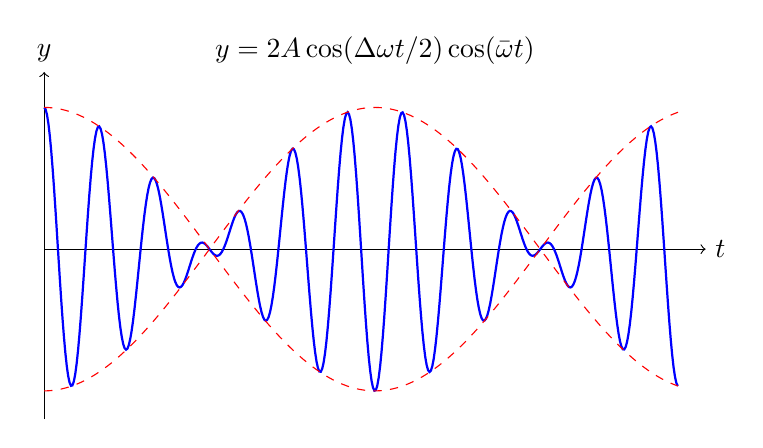
\begin{tikzpicture}[x=.7cm,y=.9cm]
\draw[->](0,0)--(12,0)node[right]{$t$};\draw[->](0,-2.4)--(0,2.5)node[above]{$y$};
\draw[blue,thick,domain=0:11.5,samples=450]plot(\x,{2*cos(30*\x)*cos(360*\x)});
\draw[red,dashed,domain=0:11.5,samples=150]plot(\x,{2*cos(30*\x)});
\draw[red,dashed,domain=0:11.5,samples=150]plot(\x,{-2*cos(30*\x)});
\node at(6,2.8){$y=2A\cos(\Delta\omega t/2)\cos(\bar\omega t)$};\end{tikzpicture}}
图\ref{fv:w3:beats}中慢变因子过零后可以变负，但可观测振幅是 $2A|\cos(\Delta\omega t/2)|$，不取负值。相邻两次强度最强的间隔因此为 $2\pi/|\Delta\omega|$，拍频为 $|f_1-f_2|$；若把不取绝对值的余弦周期直接当成拍周期，就会多一个二。两频率相差远小于平均频率时，才容易分辨快振动与慢包络。


\section{多普勒效应的发射与接收时间}
对经典声波，速度必须相对介质定义。沿从声源到接收者的传播方向取单位向量$\boldsymbol n$，设两者速度在该方向的分量为$v_S,v_D$。相邻波面发射间隔$T$，波源在这段时间前进$v_ST$，所以波面间距为$(u-v_S)T$；接收者与波面相对速度为$u-v_D$。因此
\[
T'=\frac{u-v_S}{u-v_D}T,\qquad
f'=\frac{u-v_D}{u-v_S}f.
\]
分子描述接收者遇到波面的速率，分母描述声源形成的波长。两者地位不对称，不能仅用相对速度替换。该形式用于给定传播支路、亚声速、速度在相邻波面发射接收期间可近似不变的情况。改变传播方向时，投影的符号必须一起改变。

若空气整体以速度$w$运动，应先将声源、接收者的地面速度减去$w$，声速$u$仍取相对空气的值。真空光的多普勒效应需要相对论关系，不能照搬声学公式。

\fig{fig:w3:doppler}{同一接收时刻的相邻波面：声源前进压缩间距，接收者运动改变遇波速度}{\begin{tikzpicture}

\draw[axis](-.3,0)--(6.3,0)node[right]{$x,\boldsymbol n$};\fill(1,0)circle(.07)node[below]{$S$};\fill(5,0)circle(.07)node[below]{$D$};
\foreach \xx in {2,3,4}{\draw[blue,thick](\xx,-.7)--(\xx,.7);}\draw[flow](1,1.2)--(2,1.2)node[above]{$v_S$};\draw[flow](5,1.2)--(5.9,1.2)node[above]{$v_D$};\draw[flow](3,-1.6)--(4.1,-1.6)node[right]{$u$};\draw[dim](2,-1)--(3,-1)node[midway,below]{$(u-v_S)T$};

\end{tikzpicture}}

图\ref{fig:w3:doppler}先以箭头规定这一路声波在介质中的传播方向，再沿该方向取声源和接收者的有符号速度。声源速度改变相邻波面的间距，接收者速度改变穿过这些波面的速率，两种作用进入分母和分子的原因不同。

\subsection{信号时间图与公式的适用边界}
用事件时间推导可以把分子、分母的物理作用分开。设$t=0$声源在$x=0$、接收者在$x=D>0$，两者速度为$v_S,v_D$，均相对空气取向右为正，且考察向右传播的同一支路。首个波面在$t=0$发射、$t_1$接收；第二个在$t=T$发射、$t_2$接收。图\ref{fig:w3:eventtimes}中的两条传播线应具有相同斜率，因为声音在空气中的速率都是$u$。
\fig{fig:w3:eventtimes}{两个发射事件和两个接收事件的时间关系}{\begin{tikzpicture}[scale=.88]\draw[axis](-.3,0)--(4.2,0)node[right]{$x$};\draw[axis](0,-.25)--(0,3)node[above]{$t$};\draw[world](0,0)--(.72,2.88)node[above]{$S$};\draw[world](3,0)--(3.36,2.88)node[above]{$D$};\draw[flow](0,0)--(3.1579,1.2632);\draw[flow](.3,1.2)--(3.3,2.4);\fill(0,0)circle(2pt)node[below left]{$E_0$};\fill(.3,1.2)circle(2pt)node[left]{$E_1$};\fill(3.1579,1.2632)circle(2pt)node[right]{$R_0$};\fill(3.3,2.4)circle(2pt)node[right]{$R_1$};\draw[guide](.3,1.2)--(-.4,1.2)node[left]{$T$};\draw[guide](0,1.2632)--(2.7,1.2632);\draw[guide](0,2.4)--(2.7,2.4);\draw[dim](2.5,1.2632)--(2.5,2.4)node[midway,left]{$T^{\prime}$};\end{tikzpicture}}
两个传播方程分别为
\[
ut_1=D+v_Dt_1,\qquad
u(t_2-T)=D+v_Dt_2-v_ST.
\]
第二式中的$v_ST$是第二次发射点的位置，不能用接收时的声源位置替代。两式相减并整理，得到$(u-v_D)(t_2-t_1)=(u-v_S)T$。令$T'=t_2-t_1$，就得到前述频率比。声源静止、接收者向源运动时$v_D<0$，分子增大；接收者静止、声源朝它运动时$v_S>0$，分母减小，两种情形都提高接收频率，却对应不同的波面几何。

如果源和接收者不共线，应使用每个传播支路上实际连线方向的速度投影。距离和方向在传播过程中变化明显时，需要先求迟滞发射时刻，再在相邻事件间求导；不能在任意时刻画一条当前连线就当作发射时的传播路径。基础题常给远场或短时间近似，允许把方向视为不变。

声源趋近声速时，前方相邻波面间距变小，公式分母趋零表明线性、稳态、点源等理想化会出现特殊极限。超过声速后波面可能形成包络锥，已超出本讲亚声速公式的适用范围。检查$v/u\to0$的极限，频率应回到$f$；将全部速度同加一个背景风速时，先转换到空气参考系才能保持物理一致。


\section{回声、反射与多次传播}
静止墙面反射时，墙面观察到的频率等于反射频率，反射只改变传播方向。移动接收者听回声，应先求墙面收到的频率，再按反射后的传播方向求接收频率。若反射体移动，它先充当接收者，再充当发射者，两次频移均要计算。

两面静止平行墙之间多次反射不会在每次反射时再凭空乘一个频移因子。波在空气中的频率只由最初发射时的传播方向决定，最终接收时再由末段传播方向决定。把初段、末段方向分别列出，就能避免重复计算或遗漏同频回声。

\subsection{运动反射体的两次频率转换}
设声源和最终接收者都相对空气静止，反射板沿入射方向以$V$远离声源，$|V|<u$。入射方向取向右，板先作为接收者，遇到波面的频率为$f_m=(u-V)f/u$。若反射过程在板的参考系中保持相邻波面的时间周期，板再作为向左发波的等效声源；这段传播方向已反转，板速度的有向分量应改为$-V$，故静止接收者收到
\[
f_r=\frac{u}{u+V}f_m
=f\frac{u-V}{u+V}.
\]
板远离时两次作用均使频率降低，板靠近时令$V<0$便得到升频。$V=0$恢复$f_r=f$。求低速近似时，先减去原频率，令$\varepsilon=V/u$，有
\[
\frac{f_r-f}{f}
=\frac{u-V-(u+V)}{u+V}
=-\frac{2\varepsilon}{1+\varepsilon}
=-2\varepsilon+\frac{2\varepsilon^2}{1+\varepsilon}.
\]
当$|\varepsilon|\ll1$时，最后一项为二阶小量，保留一阶得到$(f_r-f)/f\simeq-2V/u$。这里的二倍来自两段传播都受运动板影响，不是任何回声都应乘二；静止墙不会在每次反射时新增频移。

\fig{fig:w3:movingmirror}{运动板先接收、再反射；回程须重新规定传播方向}{\begin{tikzpicture}

\fill(0,0)circle(.07)node[left]{$S,D$};\draw[world](5,-1.5)--(5,1.5);\node[right]at(5,1.5){反射板};\draw[flow](5,2.1)--(6.1,2.1)node[right]{$V>0$};
\draw[flow](.5,.6)--(4.5,.6)node[midway,above]{$\boldsymbol n_+=+\boldsymbol e_x,\quad f$};\draw[flow](4.5,-.6)--(.5,-.6)node[midway,below]{$\boldsymbol n_-=-\boldsymbol e_x,\quad f_r$};\node at(2.4,-2){板接收：$v_D=V$；板再发射：$v_S=-V$};

\end{tikzpicture}}
图\ref{fig:w3:movingmirror}中板向右远离，入射波追板较慢；板再向左发出的相邻波面间距又被拉大。这两种几何变化分别给出$u-V$与$u+V$，同时造成降频。把板改为向左靠近，只需令同一有向速度$V<0$，不能在方向反转时保留错误的投影符号。


还可按相邻脉冲的飞行时间检查。设发射时板到静止声源的距离为$D$，往返时间$\tau$满足去程$ut_m=D+Vt_m$，回程$u(\tau-t_m)=D+Vt_m$，故$\tau=2D/(u-V)$。连续两次发射相隔$T$，第二次发射时初距离增加$VT$，接收间隔变为$T'=T+2VT/(u-V)=T(u+V)/(u-V)$，其倒数与波面法相同。飞行时间决定信号何时到达，飞行时间随发射时刻的变化才决定频率改变。


\section{时间相位差与空间相位差的联系}
对某一点的两列同频波，初相差不随时间改变，所以合振幅稳定；对不同频率的两列波，相位差为$(\omega_2-\omega_1)t+\Delta\varphi_0$，强弱会随时间改变。空间干涉与拍并非两套无关规则：它们都由相位差决定，只是相位差主要依赖位置还是依赖时间不同。解题应先写完整相位差，再决定把它看作空间函数还是时间函数。

若接收者沿路径$x(t)$移动，接收相位为$\psi(t)=\omega t-kx(t)+\varphi_0$，瞬时角频率是$\dd\psi/\dd t=\omega-k\dot x$。这直接给出静止声源时的接收者频移，显示运动接收者并没有改变空气中的波长。若声源运动，则要从相邻发射事件求波面间距，不能把同一相位函数中的$x(t)$同时当作声源坐标与接收者坐标。

反射回声与直接声音同时到达接收者时，还可能产生拍。先逐路求各自接收频率，若两频率接近且相位在观察时间内较稳定，拍频才是它们之差。传播时间主要影响初始相位和信号到达窗口，频移则由相邻事件间隔变化决定。长路程不必产生较大频移，静止源、静止墙和静止接收者即使多次反射，频率仍可保持不变。

声管端点的“相位反转”也要指定变量。刚性封闭端空气位移反号，而压强反射同号；开口端近似相反。同一反射过程的位移波节和压强波腹共存，不能把其中一项的半波损失照搬给另一项。处理机械位移、声压或光场干涉时，都应先说明叠加的是哪一个量。

相位采用正弦或余弦只是一种记号选择，整体移动初相不会改变可观测预测。真正需要一致的是两路之间的相对初相、每段传播方向和边界附加相位。完成复杂叠加后，检查相等振幅、零程差、两源反相以及速度趋零等极限，可以把代数结果与物理图像重新连接起来。

